\section{Test strategy}


\begin{frame}{Test pyramid}
  \begin{center}
  \begin{tikzpicture}
    \cadre
    \etoepart
    \integpart
    \unitpart
    \node [alert_color] at($ (etoe.center) + (-1.4, 0)$)  {10};
    \node [alert_color] at($ (integ.center) + (-2.5, 0)$) {100};
    \node [alert_color] at($ (unit.center) + (-3.6, 0)$)  {10000};
  \end{tikzpicture}
  \end{center}
\end{frame}


\begin{frame}{Functional vs Technical tests}
  \begin{center}
  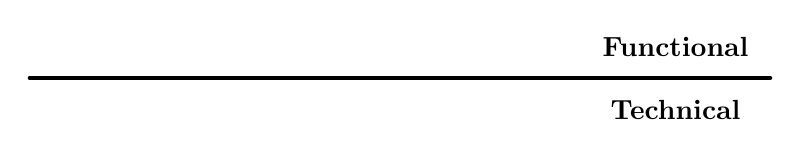
\begin{tikzpicture}
    \cadre
    \etoepart
    \integpart
    \unitpart
    \draw[ultra thick,line cap=round] (-1.7,3.9) -- (7.7,3.9);
    \node at(6.5,4.3) {\alert{\textbf{Functional}}};
    \node at(6.5,3.5) {\alert{\textbf{Technical}}};
  \end{tikzpicture}
  \end{center}
\end{frame}


\begin{frame}{Functional vs Technical tests}
  \begin{center}
  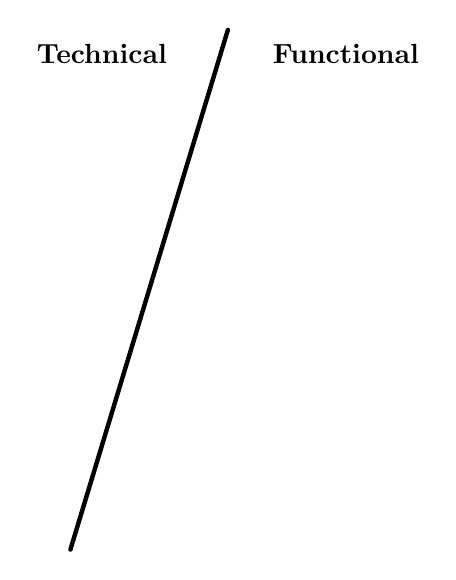
\begin{tikzpicture}
    \cadre
    \etoepart
    \integpart
    \unitpart
    \draw[ultra thick,line cap=round] (1,-0.3) -- (3,6.3);
    \node at(4.5,6) {\alert{\textbf{Functional}}};
    \node at(1.4,6) {\alert{\textbf{Technical}}};
  \end{tikzpicture}
  \end{center}
\end{frame}


\begin{frame}{Functional vs Technical tests}
  \begin{center}
  \begin{tikzpicture}
    \cadre
    \etoepart
    \integpart
    \unitpart

    \begin{scope}
      \clip (0, 0) rectangle (6,1.8);
      \clip (6,-0.3) -- (1,-0.3) -- (3,6.3) -- (6,6.3) -- cycle;
      \fill[alert_color!20!white ] (0,0) -- (6,0) -- (3,6) -- cycle;
      \node (unit) at (3,0.5) {Unit};
    \end{scope}

    \node at(4.5,6) {\alert{\textbf{Functional}}};
    \node at(1.4,6) {\alert{\textbf{Technical}}};
    \draw[ultra thick,line cap=round] (1,-0.3) -- (3,6.3);
  \end{tikzpicture}
  \end{center}
\end{frame}
